\chapter{Planarity}
\section{Planar Graphs}
(lat. planaris - flat, level)

% 5.1 Definition
\begin{definition}
A \textbf{\color{red}graph} $G=(V,E)$ is called \textbf{\color{red}planar} if it can be drawn on a plane s.t. its edges at most intersect in their end vertices. Any such drawing is then called a \textbf{\color{red}planar representation} or a \textbf{\color{red}planar embedding}. If $G$ is not planar, it is called \textbf{\color{red}nonplanar}.
\end{definition}

% 5.2 Examples
\begin{example}
\begin{enumerate}
    \item[1)] Clearly, trees, cycles and empty graphs are planar.
    \item[2)] The graph 
    \begin{center}
    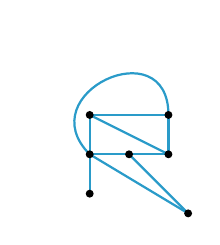
\begin{tikzpicture}[scale=0.5, thick]
        % 1. Define the coordinates (Nodes)
        % Top row
        \coordinate (TL) at (0, 2);   % Top Left
        \coordinate (TR) at (2, 2);   % Top Right

        % Middle row
        \coordinate (ML) at (0, 1);   % Mid Left
        \coordinate (MC) at (1, 1);   % Mid Center
        \coordinate (MR) at (2, 1);   % Mid Right

        % Bottom row
        \coordinate (BL) at (0, 0);       % Bottom Left
        \coordinate (BR) at (2.5, -0.5);  % Bottom Right (angled down)

        % 2. Draw the Edges (Lines)
        \begin{scope}[cyan!80!black]
            % The box and diagonals on top
            \draw (TL) -- (TR);
            \draw (TL) -- (ML);
            \draw (TR) -- (MR);
            \draw (TL) -- (MR); % Diagonal top-left to mid-right

            % The horizontal middle line
            \draw (ML) -- (MC) -- (MR);

            % The bottom connections
            \draw (ML) -- (BL); % Vertical down
            \draw (ML) -- (BR); % Long diagonal down
            \draw (MC) -- (BR); % Short diagonal down

            % The big curved line (Loop)
            % out=135 means "leave at 135 degrees", in=90 means "enter at 90 degrees"
            \draw (ML) to[out=135, in=90, looseness=2.5] (TR);
        \end{scope}

        % 3. Draw the Vertices (Dots)
        \foreach \p in {TL, TR, ML, MC, MR, BL, BR}
            \filldraw (\p) circle (2pt);

    \end{tikzpicture}
    \end{center}
    is planar and this is a planar representation:
    

    \item[3)] The graph $K_{2,3}$
    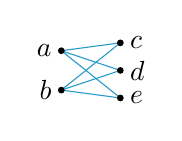
\begin{tikzpicture}[baseline=(current bounding box.center), scale=0.5]
        \coordinate (a) at (0,1); \node[left] at (a) {$a$};
        \coordinate (b) at (0,0); \node[left] at (b) {$b$};
        \coordinate (c) at (1.5,1.2); \coordinate (d) at (1.5,0.5); \coordinate (e) at (1.5,-0.2);
        \node[right] at (c) {$c$}; \node[right] at (d) {$d$}; \node[right] at (e) {$e$};
        
        \foreach \x in {a,b} \foreach \y in {c,d,e} \draw[cyan!80!black] (\x)--(\y);
        \foreach \p in {a,b,c,d,e} \filldraw (\p) circle (2pt);
    \end{tikzpicture}
    is planar, but this is not a planar representation. One planar representation is given by
    \begin{center}
    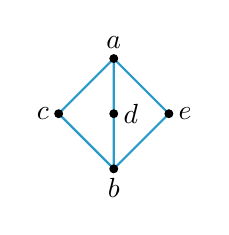
\begin{tikzpicture}[scale=0.7]
        \coordinate (a) at (0,1); \node[above] at (a) {$a$};
        \coordinate (b) at (0,-1); \node[below] at (b) {$b$};
        \coordinate (d) at (0,0); \node[right] at (d) {$d$};
        \coordinate (c) at (-1,0); \node[left] at (c) {$c$};
        \coordinate (e) at (1,0); \node[right] at (e) {$e$};
        
        \draw[cyan!80!black, thick] (a)--(c)--(b)--(d)--(a)--(e)--(b);
        \foreach \p in {a,b,c,d,e} \filldraw (\p) circle (2pt);
    \end{tikzpicture}
    \end{center}
\end{enumerate}
\end{example}

In order to prove that a graph is planar, we ``just'' have to provide one planar representation. But these can be very hard to find.
In order to prove that a graph is \underline{not} planar, we would have to check ``all'' possible representations. This is not feasible.

But we can help ourselves by throwing some math on the problem.
To this end, we need some more terminology.

% 5.3 Definition
\begin{definition}
A \textbf{\color{red}region} in a planar rep. is a maximal area of the plane s.t. any two points within can be connected by a curve which does not intersect or touch any part of the graph.
Regions which are completely bounded (= surrounded) by graph edges are called \textbf{\color{red}interior regions}. The unique non-interior region is called \textbf{\color{red}exterior region}.
\end{definition}

% 5.4 Example
\begin{example}
Consider the planar representation
\begin{center}
    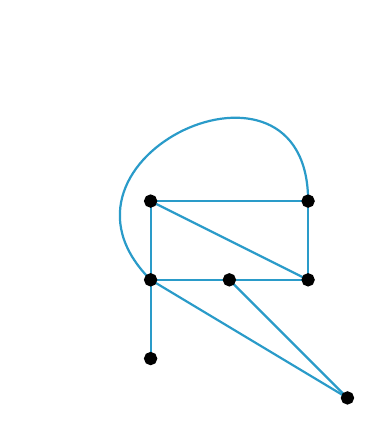
\begin{tikzpicture}[scale=1, thick]
        % 1. Define the coordinates (Nodes)
        % Top row
        \coordinate (TL) at (0, 2);   % Top Left
        \coordinate (TR) at (2, 2);   % Top Right

        % Middle row
        \coordinate (ML) at (0, 1);   % Mid Left
        \coordinate (MC) at (1, 1);   % Mid Center
        \coordinate (MR) at (2, 1);   % Mid Right

        % Bottom row
        \coordinate (BL) at (0, 0);       % Bottom Left
        \coordinate (BR) at (2.5, -0.5);  % Bottom Right (angled down)

        % 2. Draw the Edges (Lines)
        \begin{scope}[cyan!80!black]
            % The box and diagonals on top
            \draw (TL) -- (TR);
            \draw (TL) -- (ML);
            \draw (TR) -- (MR);
            \draw (TL) -- (MR); % Diagonal top-left to mid-right

            % The horizontal middle line
            \draw (ML) -- (MC) -- (MR);

            % The bottom connections
            \draw (ML) -- (BL); % Vertical down
            \draw (ML) -- (BR); % Long diagonal down
            \draw (MC) -- (BR); % Short diagonal down

            % The big curved line (Loop)
            % out=135 means "leave at 135 degrees", in=90 means "enter at 90 degrees"
            \draw (ML) to[out=135, in=90, looseness=2.5] (TR);
        \end{scope}

        % 3. Draw the Vertices (Dots)
        \foreach \p in {TL, TR, ML, MC, MR, BL, BR}
            \filldraw (\p) circle (2pt);

    \end{tikzpicture}
    \end{center}

We can find the regions by considering this representation as a cookie cutter which we use to part the dough on our table surface.
So the regions are:

\begin{center}
    \includegraphics[width=0.6\textwidth]{./images/pic_5_4.png}
\end{center}
where $R_1-R_4$ are interior and $R_5$ is the exterior region.
\end{example}

% 5.5 Definition
\begin{definition}
Let $\Gamma$ be a planar representation of $G$ in $\mathbb{R}^2$. We say that an edge $e$ is \textbf{\color{red}incident} with a region $R$ iff every point $x$ on the edge $e$ and $\varepsilon > 0$ there is a point $y$ in $R$ s.t. $d(x,y) < \varepsilon$ (or $B_\varepsilon(x) \cap R \ne \emptyset$). We say that $e$ is a \textbf{\color{red}bound} for $R$, if it is incident with $R$ and at least one other region. We denote the number of bounds for a given region $R$ by \textbf{\color{red}$b(R)$} and call it its \textbf{\color{red}boundary degree} while $B(R) = \{e \in E(G) \mid e \text{ is a bound for } R\}$ is called the \textbf{\color{red}boundary} of $R$.
\end{definition}

% 5.6 Example
\begin{example}
Consider $G$ given by its planar representation
\begin{center}
\begin{tikzpicture}[scale=1.2, thick]

    % --- 1. Define Coordinates ---
    % Outer Triangle
    \coordinate (A) at (-3, 0);   % Bottom Left
    \coordinate (B) at (3, 0);    % Bottom Right
    \coordinate (C) at (0, 4);    % Top Center

    % Vertical Spine (Top Extension)
    \coordinate (D) at (0, 5.5);  % Very Top Point

    % Inner Triangle
    \coordinate (E) at (0, 2);    % Inner Top
    \coordinate (F) at (-0.8, 1.2); % Inner Bottom Left
    \coordinate (G) at (0.8, 1.2);  % Inner Bottom Right

    % The node between Inner Top (E) and Outer Top (C)
    \coordinate (H) at (0, 3);

    % --- 2. Draw Regions Text (Background) ---
    \node[scale=1.2] at (0, 1.5) {$R_1$};
    \node[scale=1.5] at (-1.5, 0.5) {$R_2$};
    \node[scale=2] at (-3.5, 3) {$R_3$};

    % --- 3. Draw The Grey Ball B_epsilon(x) ---
    % Calculate a point 'x' halfway along edge e3 (between A and C)
    \coordinate (X) at ($(A)!0.4!(C)$); 
    
    % Draw the circle
    \draw[gray!60, thick] (X) circle (0.35cm);
    % Draw the label
    \node[gray!80, font=\small, anchor=south east] at ($(X)+(-0.1, 0.1)$) {$B_\varepsilon(x)$};
    % Draw the point x
    \filldraw[gray] (X) circle (1.5pt) node[right, black, scale=0.7] {$x$};


    % --- 4. Draw Edges and Labels ---
    \begin{scope}[cyan!80!black]
        % Outer Triangle Edges
        \draw (A) -- node[below, red, scale=1.2, yshift=-2pt] {$e_1$} (B);
        \draw (B) -- node[above right, red, scale=1.2] {$e_2$} (C);
        \draw (C) -- node[above left, red, scale=1.2] {$e_3$} (A);

        % Inner Triangle Edges
        \draw (F) -- node[below, red, scale=1.2, yshift=-2pt] {$e_4$} (G);
        \draw (G) -- node[right, red, scale=1.2, xshift=2pt] {$e_5$} (E);
        \draw (E) -- node[left, red, scale=1.2, xshift=-2pt] {$e_6$} (F);

        % Vertical Spine Edges
        \draw (E) -- node[right, red, scale=1.2] {$e_7$} (H);
        \draw (H) -- node[right, red, scale=1.2] {$e_8$} (C);
        \draw (C) -- node[right, red, scale=1.2] {$e_9$} (D);
    \end{scope}

    % --- 5. Draw Vertices ---
    \foreach \p in {A,B,C,D,E,F,G,H}
        \filldraw (\p) circle (2pt);

\end{tikzpicture}
\end{center}
Then $e_6$ is a bound of $R_2$, as it is incident with $R_1$ and $R_2$, but $e_7$ is not a bound of $R_2$, as it is only incident with $R_2$.
Further, $B(R_2) = \{e_1, e_2, e_3, e_4, e_5, e_6\}$ and $b(R_2)=6$. Also, $B(R_3) = \{e_1, e_2, e_3\}$ and $B(R_1) = \{e_4, e_5, e_6\}$.
\end{example}

% 5.7 Remarks
\begin{remark}
\begin{itemize}
    \item A very proper treatment needs a good fusion of real analysis with topology and exceeds our time frame (nice thesis topic).
    \item Any edge is incident with either 1 or 2 regions, whence
    \[ \sum b(R) = \sum |B(R)| = 2 |\{e \mid e \text{ is a bound for some } R \}| \le 2|E|. \]
    \item Any region either has no bounds or at least three.
    \item A region has no bound iff it is the only region and $G$ is a forest.
\end{itemize}
\end{remark}

% 5.9 Fact
\topic{Fact}
Assume $\Gamma$ is the planar representation of a graph $G$ with regions $R_1, R_2, \dots, R_r$. Then
\begin{enumerate}
    \item[1)] Either $G$ is a forest and $r=1$ and $b(R_1)=0$ or
    \item[2)] $G$ contains a cycle and $r \ge 2$ with
    \[ 3r \le \sum_{i=1}^r b(R_i) \le 2|E|. \]
\end{enumerate}

% 5.10 Observation
\topic{Observation}
Let $e$ be the edge of a planar graph $G$. Then $e$ is a bound for some region $R$ iff $e$ is part of a cycle in $G$.

We now will prove that the relation discovered in the intermezzo holds for \underline{any} planar representation.

% 5.11 Theorem (Euler's Formula)
\begin{theorem}[Euler's Formula]
Let $\Gamma$ be any planar representation of a connected graph $G$. Then for $|G|=n, \|G\|=m$ and $r$ the number of regions in $\Gamma$, we have
\[ \boxed{n - m + r = 2.} \]
\end{theorem}

% 5.12 Corollaries
\begin{theorem}[Corollaries]
    \begin{enumerate}
        \item[1)] As consequently $r = \|G\| - |G| + 2$, we get that for a planar graph $G$, the number of regions is independent from the chosen planar representation. We can hence say that $G$ has $r$-many regions.
        \item[2)] If $G$ is a planar graph on $k$-many connected components $C_1 \dots C_k$ then each $C_i$ is planar. If $C_i$ has $r_i$-many regions, note that $G$ has $\sum_{i=1}^k r_i - (k-1)$ many regions as all components share the common exterior region in a joint embedding. Thus the number of regions $r$ of $G$ is
        \[ r = (\sum r_i) - (k-1) = \sum (\|C_i\| - |C_i| + 2) - (k-1) \]
        \[ = \|G\| - |G| + 2k + 1 = \|G\| - |G| + k + 1. \]
        Hence, for arbitrary planar $G$ with $|G|=n, \|G\|=m$ and $\rho(G)=r$, we get
        \[ \boxed{n - m + r = k+1} \]
    \end{enumerate}
\end{theorem}


\begin{proof}[Proof of Theorem 5.11]
Let $G$ be a connected planar graph in any given planar representation with regions $R_1, R_2, \dots, R_r$. Let $|G|=n$.
We prove the theorem by induction on $\|G\|=m$.

\vspace{0.3cm}
\noindent \underline{$m=0$:} If $G$ has no edges, then $G=K_1$. Then clearly $n=1, r=1$ and thus $n-m+r = 1-0+1 = 2$, as desired.

\vspace{0.3cm}
\noindent \underline{$m-1 \to m$:} Assume we established the claim for all graphs with less than $m$ many edges. Consider $G$ with $m$ many edges.
If $G$ is a tree, then we know that $n=m+1$ and $r=1$ (whence $n-m+r = m+1-m+1=2$, as desired).
Otherwise, $G$ contains at least one cycle. Let $e \in E(G)$ be one edge on that cycle. Then by Observation 5.10, $e$ is a bound for two regions $R_i$ and $R_j$. Note that in $G-e$ the regions $R_i$ and $R_j$ merge together to one new region $R'$, whence $G-e$ has one less region than $G$. Thus, by I.H. we get
\[ |G-e| - \|G-e\| + (r-1) = n - (m-1) + (r-1) = n - m + r, \text{ as desired.} \qedhere \]
\end{proof}

% 5.13 Remark
\begin{remark}
\begin{enumerate}
    \item[1)] Every subgraph of a planar graph is planar.
    \item[2)] If $G$ is planar and $R$ is any region, then in the induced planar representation for $B(R)$ (i.e. deleting all drawings apart from $B(R)$), $R$ is still a region and $B(R)$ its boundary.
    \item[3)] For any region we have $b(R) \in \{0\} \cup \mathbb{N}_{\ge 3}$. In particular, if $b(R)=3$, then $B(R) \cong C_3$.
\end{enumerate}
\end{remark}

\section{Nonplanar Graphs}

Imagine you want to connect three houses each to gas, electricity and water, s.t. the pipes don't intersect. This question boils down to asking: Is the utility graph $K_{3,3}$ a planar graph?

\begin{center}
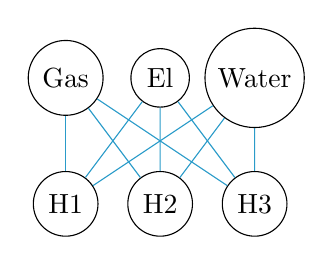
\begin{tikzpicture}[scale=0.8]
    \node[draw, circle] (gas) at (0,2) {Gas};
    \node[draw, circle] (el) at (1.5,2) {El};
    \node[draw, circle] (wat) at (3,2) {Water};
    
    \node[draw, circle] (h1) at (0,0) {H1};
    \node[draw, circle] (h2) at (1.5,0) {H2};
    \node[draw, circle] (h3) at (3,0) {H3};
    
    \draw[cyan!80!black] (gas)--(h1); \draw[cyan!80!black] (gas)--(h2); \draw[cyan!80!black] (gas)--(h3);
    \draw[cyan!80!black] (el)--(h1); \draw[cyan!80!black] (el)--(h2); \draw[cyan!80!black] (el)--(h3);
    \draw[cyan!80!black] (wat)--(h1); \draw[cyan!80!black] (wat)--(h2); \draw[cyan!80!black] (wat)--(h3);
\end{tikzpicture}
\end{center}
(This is why $K_{3,3}$ is also called the \textbf{\color{red}utility graph}.)

% 5.14 Theorem
\begin{theorem}
The utility graph $K_{3,3}$ is not planar.
\end{theorem}

\begin{proof}
Aiming for a contradiction, assume $K_{3,3}$ was planar. Then it needed to have $r = \|K_{3,3}\| - |K_{3,3}| + 2 = 9 - 6 + 2 = 5$ regions. On the other hand, as $K_{3,3}$ is bipartite and thus does not contain odd cycles, every region has at least four bounds by Remark 5.13(3). Hence
\[ \sum_{i=1}^5 b(R_i) \ge 5 \cdot 4 = 20 > 2 \cdot 9 = 2 \cdot \|K_{3,3}\|, \]
contradicting Fact 5.9.
Thus, $K_{3,3}$ cannot be planar.
\end{proof}

% 5.15 Theorem
\begin{theorem}
Let $G$ be planar of order at least 3. Then $\|G\| \le 3(|G|-2)$.
Further, if equality holds then every region is bounded by exactly three edges.
\end{theorem}

\begin{proof}
Assume $G$ consists of $k$ connected components. The equation clearly holds for forests as then $\|G\| = |G|-k \le 3|G|-6$ iff $6-k \le 2|G|$.
Otherwise, $r \ge 2$ and $G$ contains a cycle. Recall that
\[ (*) 3 \cdot r \le \sum b(R_i) \le 2\|G\|. \]
Hence, by Euler's generalised formula, we get $r = \|G\| - |G| + k+1 \ge \|G\| - |G| + 2$. This yields
\[ 2\|G\| \ge 3r \ge 3(\|G\| - |G| + 2), \text{ whence } 3(|G|-2) \ge \|G\|, \text{ as desired.} \]
Finally, for equality to hold we need in particular that $2\|G\| = 3r$, whence also $3r = \sum b(R_i)$. Thus, every region has boundary degree 3 as desired.
\end{proof}

% 5.16 Corollary
\begin{corollary}
The complete graph $K_n$ is planar iff $n \le 4$.
\end{corollary}

\begin{proof}
First note that $K_4 =$ 
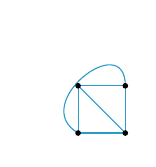
\begin{tikzpicture}[baseline=-0.5ex, scale=0.4]
    % 1. Define Coordinates
    \coordinate (TL) at (0, 1.5); % Top Left
    \coordinate (TR) at (1.5, 1.5); % Top Right
    \coordinate (BL) at (0, 0);   % Bottom Left
    \coordinate (BR) at (1.5, 0); % Bottom Right

    % 2. Draw the Edges
    \begin{scope}[cyan!80!black]
        % The outer square
        \draw (TL) -- (TR) -- (BR) -- (BL) -- (TL);
        
        % The straight diagonal (inside)
        \draw (TL) -- (BR);
        
        % The curved diagonal (outside)
        % out=150: leaves Bottom-Left going up-left
        % in=90: enters Top-Right from the top
        % looseness=2: makes the loop wide enough to go around the Top-Left node
        \draw (BL) to[out=150, in=90, looseness=2.2] (TR);
    \end{scope}

    % 3. Draw the Vertices
    \foreach \p in {TL, TR, BL, BR}
        \filldraw (\p) circle (2pt);
\end{tikzpicture}
is planar, and hence so are its subgraphs $K_1, K_2$ and $K_3$.
Now, for $K_5$, by Lemma 5.15 we get $10 = \|K_5\| \le 3(\|K_5\|-2) = 3(3) = 9$, a contradiction. Hence, $K_5$ is not planar and so is neither of the $K_n$ for $n \ge 5$, as they contain $K_5$ as a subgraph.
\end{proof}

% 5.17 Theorem
\begin{theorem}
If $G$ is planar, then $\delta(G) \le 5$.
\end{theorem}

\begin{proof}
Let $G$ be a planar graph and set $n=|G|$ and $m=\|G\|$. Aiming for a contradiction, assume $\delta(G) > 5$. Then in particular, $n \ge 6$. Then
\[ 6 \cdot n \le \sum_{v \in V_G} \deg(v) = 2m \overset{(5.15)}{\le} 2(3(n-2)) = 6n - 12 \]
yields a contradiction.
\end{proof}

\section{Kuratowski's Theorem}

We have seen that the graphs $K_{3,3}$ and $K_5$ are not planar. It turns out that these two graphs are the major obstruction for any graph to be planar. This section gives an introduction to Kuratowski's theorem. But first, we want to introduce a new notation.

% 5.18 Example
\begin{example}
Consider
\begin{center}
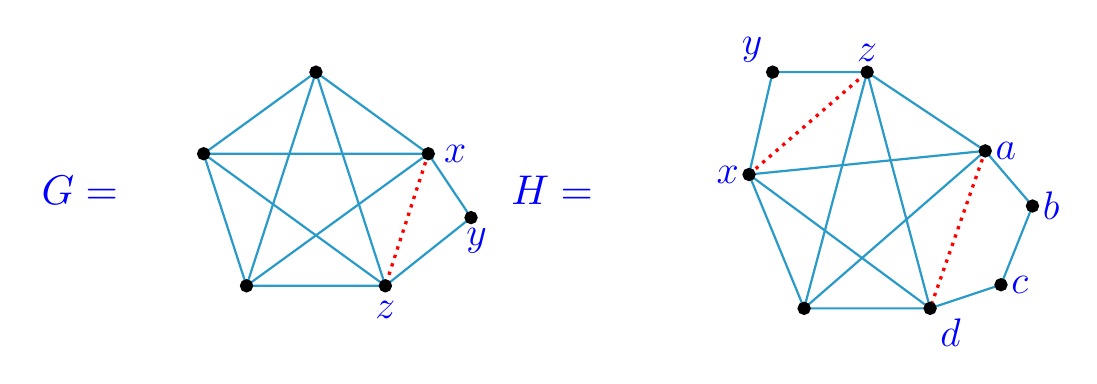
\begin{tikzpicture}[scale=1, thick]

    % ================= GRAPH G (Left) =================
    \begin{scope}[shift={(-4,0)}]
        % 1. Define Vertices (Regular Pentagon layout)
        \coordinate (g_top) at (90:1.5);
        \coordinate (g_tl)  at (162:1.5);
        \coordinate (g_bl)  at (234:1.5);
        \coordinate (g_br)  at (306:1.5); % This is y
        \coordinate (g_tr)  at (18:1.5);  % This is x
        \coordinate (extra)  at (350:2);

        % Labels for G vertices (based on your sketch)
        \node[right, blue, xshift=2pt] at (g_tr) {\Large $x$};
        \node[below, blue, xshift=2pt] at (extra) {\Large $y$};
        \node[below, blue, yshift=-2pt] at (g_br) {\Large $z$};

        % 2. Draw standard K5 edges (Cyan)
        % We draw all edges EXCEPT the red dashed one (x to z = g_tr to g_bl)
        \draw[cyan!80!black] (g_top)--(g_tl)--(g_bl)--(g_br)--(extra)--(g_tr)--(g_top); % Pentagon
        \draw[cyan!80!black] (g_top)--(g_bl) (g_top)--(g_br);
        \draw[cyan!80!black] (g_tl)--(g_br) (g_tl)--(g_tr);
        \draw[cyan!80!black] (g_tr)--(g_bl); % x to z


        % 3. Draw the special Red Dotted edge (x to z)
        \draw[red, dotted, very thick] (g_tr) -- (g_br);

        % 4. Draw Vertices dots
        \foreach \p in {g_top, g_tl, g_bl, g_br, g_tr, extra}
            \filldraw (\p) circle (2pt);

        % Label "G ="
        \node[blue, scale=1.5] at (-3, 0) {$G=$};
    \end{scope}


    % ================= GRAPH H (Right) =================
    \begin{scope}[shift={(3,0)}]
        % 1. Define Main "K5" Vertices (distorted to match sketch)
        \coordinate (z) at (0, 1.5);      % Top
        \coordinate (x) at (-1.5, 0.2);   % Mid Left
        \coordinate (w) at (-0.8, -1.5);  % Bottom Left
        \coordinate (d) at (0.8, -1.5);   % Bottom Right
        \coordinate (a) at (1.5, 0.5);    % Top Right

        % 2. Define Subdivision Vertices (bulging out)
        \coordinate (y) at (-1.2, 1.5);   % Between x and z
        \coordinate (b) at (2.1, -0.2);   % Between a and d (upper)
        \coordinate (c) at (1.7, -1.2);   % Between a and d (lower)

        % Labels
        \node[left, blue] at (x) {\Large $x$};
        \node[above left, blue] at (y) {\Large $y$};
        \node[above, blue] at (z) {\Large $z$};
        \node[right, blue] at (a) {\Large $a$};
        \node[right, blue] at (b) {\Large $b$};
        \node[right, blue] at (c) {\Large $c$};
        \node[below right, blue] at (d) {\Large $d$};

        % 3. Draw Edges
        % --- The Red Dotted "Original" Edges ---
        \draw[red, dotted, very thick] (x) -- (z);
        \draw[red, dotted, very thick] (a) -- (d);

        % --- The Solid Cyan Edges ---
        \begin{scope}[cyan!80!black]
            % Subdivision paths (Outer)
            \draw (x) -- (y) -- (z);
            \draw (a) -- (b) -- (c) -- (d);
            
            % Bottom connection
            \draw (x) -- (w) -- (d);
            
            % Internal K5 connections (The star)
            \draw (z) -- (w);
            \draw (z) -- (d);
            \draw (z) -- (a);
            
            \draw (x) -- (d);
            \draw (x) -- (a); % This crosses z-w
            
            \draw (w) -- (a);
        \end{scope}

        % 4. Draw Vertices dots
        \foreach \p in {x,y,z,a,b,c,d,w}
            \filldraw (\p) circle (2pt);

        % Label "and H ="
        \node[blue, scale=1.5] at (-4, 0) {$H=$};
    \end{scope}

\end{tikzpicture}
\end{center}
Note that neither of $G$ or $H$ contains $K_5$ (or $K_{3,3}$) as a subgraph. Nevertheless, they both look so similar to $K_5$ that they should not be planar.
Indeed, $G$ arises from $K_5$ by replacing the edge $xz$ by $\{xy, yz\}$ and $H$ arises from $G$ by replacing the edges $\{xz, ad\}$ by $\{xy, yz, ab, bc, cd\}$. This process is called subdivision.
\end{example}

% 5.19 Definition
\begin{definition}
\begin{enumerate}
    \item[1)] Let $G$ be a graph and $e=xy \in E(G)$. An \textbf{\color{red}edge subdivision} of $e$ is the replacement of $e$ by a finite path of length $\ge 2$ starting in $x$ and ending in $y$.
    \item[2)] Let $G$ and $H$ be graphs. Then $H$ is called a \textbf{\color{red}subdivision} of $G$ iff $H$ can be obtained through a finite sequence of edge subdivisions.
\end{enumerate}
\end{definition}

% 5.20 Examples
\begin{example}
\begin{enumerate}
    \item[1)] The graphs $G, H$ from 5.18 are edge subdivisions of $K_5$.
    \item[2)] The graph 
    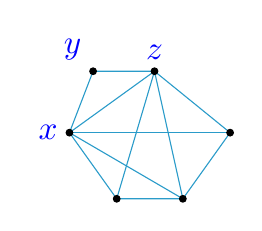
\begin{tikzpicture}[baseline=(current bounding box.center), scale=0.6]
        % 1. Define Coordinates
        \coordinate (z)  at (0.6, 1.5);      % Top right-ish
        \coordinate (y)  at (-0.7, 1.5);   % Top left-ish
        \coordinate (x)  at (-1.2, 0.2);   % Left
        \coordinate (bl) at (-0.2, -1.2);  % Bottom Left
        \coordinate (br) at (1.2, -1.2);   % Bottom Right
        \coordinate (r)  at (2.2, 0.2);    % Far Right

        % 2. Draw Edges (Cyan)
        \begin{scope}[cyan!80!black]
            % The top triangle cluster
            \draw (x) -- (y) -- (z) -- (x);

            % The fan from z to the other nodes
            \draw (z) -- (r);
            \draw (z) -- (br);
            \draw (z) -- (bl);

            % The bottom/outer connections
            \draw (x) -- (bl) -- (br) -- (r);

            % The horizontal crossing line
            \draw (x) -- (r);
            \draw (x) -- (br);
        \end{scope}

        % 3. Draw Vertices (Black dots)
        \foreach \p in {x,y,z,bl,br,r}
            \filldraw (\p) circle (2pt);

        % 4. Labels
        \node[left, blue, scale=1.2] at (x) {$x$};
        \node[above left, blue, scale=1.2] at (y) {$y$};
        \node[above, blue, scale=1.2] at (z) {$z$};
    \end{tikzpicture}
    is \textbf{\color{red}not} an edge subdivision of $K_5$, as the edges $\{xy, yz\}$ were added rather than replacing the edge $xz$.
\end{enumerate}
\end{example}

% 5.21 Lemma
\begin{lemma}
A graph $G$ is planar iff every subdivision of $G$ is planar.
\end{lemma}

\begin{proof}
``$\Rightarrow$'' Consider a planar representation $\Gamma$ of $G$. Let $H$ be a subdivision of $G$ where a sequence of $n$-many edge subdivisions were performed. We do induction on $n$.

\vspace{0.3cm}
If $n=0$, then $H=G$ is clearly planar.

\vspace{0.3cm}
Now assume we proved the claim for $n$ and consider $H$ arising from $G$ through $n+1$ many subdivisions. Let $H_0$ be the graph arising from $G$ through the first $n$-many subdivisions. By I.H. $H_0$ is planar and $H$ can be obtained from $H_0$ through exactly one edge-subdivision. Let $\Gamma_0$ be a planar drawing of $H_0$ and $e=xy$ be the edge which is subdivided to obtain $H$, say by replacing it by the path $P=(x=x_0, x_1, \dots, x_k=y)$ for $k \ge 2$. Let $\vec{xy}$ be the geodesic from $x$ to $y$ in $\mathbb{R}^2$. Then we draw in the vertex $x_i$ at the point $x + \frac{i}{k}\vec{xy}$ for any $i$. This yields a planar representation of $H$, as desired.
\end{proof}

% 5.22 Corollary
\begin{corollary}
If $G$ contains a subdivision of $K_{3,3}$ or $K_5$ as a subgraph, then $G$ is not planar. (Or: If $G$ planar $\Rightarrow$ no subdivision of $K_5, K_{3,3} \subseteq G$)
\end{corollary}

% 5.23 Theorem (Kuratowski's Theorem)
\begin{theorem}[Kuratowski's Theorem]
A graph is planar if and only if it does not contain a subdivision of $K_{3,3}$ or $K_5$ as a subgraph.
\end{theorem}

% 5.24 Remark
\begin{remark}
The left over, hard direction is the backwards direction, i.e. if $G$ does not contain a subdivision of $K_{3,3}$ or $K_5$, then $G$ is planar.
\end{remark}